\typeout{NT FILE marrow_graph.tex}%

\chapter{Marrow-Graph}


In this chapter we present the design and implementation of Marrow-Graph, a fast \gls{GPU}-accelerated dynamic graph processing library, which includes a set of commonly used graph processing algorithms and allows for efficient graph manipulations.

\section{Programming Model \& Interface}

\begin{listing}%[H]
\begin{minted}
[
frame=lines,
linenos,
fontsize=\scriptsize
]
{cpp}
template<typename vertex_attributes>
struct vertex {
    idx_t idx;
    std::size_t degree;
    idx_t adjacency_list;
    idx_t adjacency_list_end;
    vertex_attributes attributes;
};

template<typename edge_attributes>
struct edge {
    idx_t dst;
    edge_attributes attributes;
};

template <typename vertex_attributes, typename edge_attributes>
class graph {

    using Vertex = vertex<vertex_attributes>;
    using Edge = edge<edge_attributes>;
public:
    virtual idx_t add_vertex(vertex_attributes attributes) = 0;
    virtual bool remove_vertex(idx_t idx) = 0;
    virtual bool add_edge(idx_t src, idx_t dst, edge_attributes attributes) = 0;
    virtual bool add_edge_batch(edge_insertion_batch<edge_attributes>& batch) = 0;
    virtual bool remove_edge(idx_t src, idx_t dst) = 0;
    virtual bool remove_edge_batch(edge_deletion_batch<edge_attributes>& batch) = 0;
    virtual bool edit_edge(idx_t src, idx_t dst, idx_t new_dst) = 0;
    virtual vector<idx_t> get_connection(idx_t idx) = 0;
    virtual std::size_t get_degree(idx_t idx) = 0;
    virtual std::size_t get_number_of_vertex() = 0;
    virtual std::size_t get_number_of_edges() = 0;
    virtual void sort() = 0;

    template <typename compute_fun, typename... compute_args>
    vector<idx_t> advance(vector<idx_t>& frontier, compute_fun& cfun, compute_args&... cargs);
    
    template <typename filter_fun, typename... filter_args>
    vector<idx_t> filter(vector<idx_t> &frontier, filter_fun& ffun, filter_args&... fargs);
};
\end{minted}
\center
\caption{Graph interface.}
\label{lst:graph_interface}
\end{listing}

We will start by defining Marrow-Graph's programming model. Our goal while designing this model was to provide an interface that was as simple and expressive as possible. As discussed in section~\ref{sec:programming_models},  bulk-synchronous is the most natural model for \gls{GPU} applications. More specifically, we believe that Gunrock's~\cite{paper:gunrock} programming model fits our purposes well. It allows one to highly optimize the small set of operations, and facilitate the development of algorithms utilizing these simple but fast operations. Another obvious benefit lies in the fact that Gunrock is an open-source project which already offers a wide array of algorithms implemented using this programming model.

% Graph abstraction
% abstraction  allows for the future experimentation with different data structures
% templated vertex attributes and templated edge attributes

All the graph manipulations and operations are performed through an abstract interface which hides the internal implementation. As we can see in listing~\ref{lst:graph_interface}, three structs are provided. The \texttt{vertex} struct includes a vertex's ID, its degree, pointers to the start and end of its adjacency list, and a templated field for storing custom vertex attributes. The \texttt{edge} struct includes the ID of the destination vertex (the source vertex is implied), and a templated field for storing custom edge attributes. Finally, the \texttt{graph} class offers a set of methods for manipulating and queering the graph, as well as the advance and filter operators.

%\paragraph{\textbf{Updates}.}
Regarding graph manipulation functions, we offer a method to create a new vertex which returns the ID of the generated vertex. Then using the generated IDs, the user can invoke the methods to remove a vertex, add an edge, remove and edge, and edit an edge. Additionally, an \texttt{add\_edge\_batch} method and a \texttt{remove\_edge\_batch} method are provided to perform optimized insertions and deletions of batched edges. As seen in listing~\ref{lst:edge_insertion_batch}, an edge batch is composed by a \texttt{std::map}, whose key is the ID of a source vertex, and value is a vector of outgoing edges. This allows marrow-graph to perform edge insertions and deletions optimally by iterating over consecutive edges that share the same source vertex.



\begin{listing}%[H]
\begin{minted}
[
frame=lines,
linenos,
fontsize=\scriptsize
]
{cpp}
template<typename edge_attributes>
struct edge_insertion_batch {
    std::size_t size;
    std::map<idx_t, std::vector<edge<edge_attributes>>> edges;

    void add(idx_t src, idx_t dst, edge_attributes attributes) { ... }
};
\end{minted}
\center
\caption{Edge Insertion Batch.}
\label{lst:edge_insertion_batch}
\end{listing}

\subsection{Operators}

%\paragraph{\textbf{Operators}.}
Similarly to Gunrock~\cite{paper:gunrock}, marrow-graph provides four main operators: advance, filter, compute and segmented intersection. As previously mentioned~\ref{gpu_graph_processing}, the compute operator can be used together with the other traversal operators. For this reason, instead of having a dedicated compute operator, each transversal method takes a compute operator as input as well as any necessary compute arguments. Besides the compute operator, all the operators receive an input frontier and return the corresponding result frontier. These frontiers are represented as a marrow vector of vertex IDs. The absence of a dedicated segmented intersection operator will be discussed later.

\paragraph{\textbf{Advance}.}
The \texttt{advance} method receives as input a templated compute function and its corresponding arguments (expressed with a variadic template). The \texttt{compute\_fun} type must be a functor whose function call operator \texttt{()} follows the following signature: \texttt{void operator()(Vertex\& sv, Vertex\& dv, Edge\& e, Args\&...) \{ ... \}}. Remember that the advance operator traverses all the outgoing edges of the vertices from the input frontier. The compute function describes the operation that is performed over a single outgoing edge, and Marrow-graph then ensures that this function is applied over every traversed edge during advance. The parameters \texttt{sv}, \texttt{dv} and \texttt{e} represent a single outgoing edge. \texttt{sv} contains the data and attributes of the source vertex, \texttt{dv} contains the data and attributes of the destination vertex, and \texttt{e} contains the attributes of the edge connecting these vertices. Besides these three arguments, the compute function can also receive and operate over any number of auxiliary arguments. These arguments must either be marrow containers or basic data types. Note however, that although the auxiliary arguments we pass to the \texttt{advance} function can be marrow containers, the type of the arguments of the \texttt{cfun} function must be their kernel type counterparts, similarly to how we define and use marrow functions. For example, we might pass a \texttt{vector<int>} as an auxiliary argument to advance, but receive a \texttt{int*} in the \texttt{cfun}. Given that the advance operator is executed on the device, the device code must operate over basic data types rather than complex marrow containers.

Listing~\ref{lst:advance_example} shows an example of how the advance operator might be used to compute the sum of the weights of all the outgoing edges of a given vertex. For the sake of simplicity, we'll assume this graph hasn't been subjected to vertex deletions which could affect the required size of the \texttt{weights} container. In lines 14-16 we start by instantiating a graph \texttt{g} and a vector \texttt{weights} with all values initialized to 0. In lines 18-19 we define a frontier with a single vertex (the vertex whose neighbor weights we'll be summing). In line 20 we call the advance operator over the frontier, passing it an instance of the \texttt{compute\_total\_weight\_fun} functor and the \texttt{weights} vector. Looking at lines 7-12, we can see that this functor follows the previous signature rules, and simply atomically sums an edge's weight to \texttt{weights} array at the index corresponding to the destination vertex. This means that after the advance operator finishes, \texttt{weights} will contain all the weights of the outgoing edges in the corresponding positions of the destination vertices . All the other positions of the container will remain equal to 0. Finally in line 22 we sum all the values of \texttt{weights} with a marrow reduce, and obtain the total sum of weights. For now we'll ignore line 21 which deals with a peculiarity of marrow.

\begin{listing}%[H]
\begin{minted}
[
frame=lines,
linenos,
fontsize=\scriptsize
]
{cpp}
struct vertex_attribute {};

struct edge_attribute {
    int weight;
};

struct compute_total_weight_fun {
    __device__
    void operator()(Vertex &src, Vertex &dst, Edge &edge, int* weights) {
        marrow::atomic::add(&weights[dst.idx], edge.weight);
    }
};

graph<vertex_attribute, edge_attribute> g = ...;
vector<int> weights(g.get_number_of_vertex());
fill(weights, 0);

idx_t vertex_id = ...;
vector<idx_t> frontier = { vertex_id };
vector<idx_t> advanced_frontier = g.advance(frontier, compute_total_weight_fun(), weights);
set_replica_dirty(weights);
int total_weight = reduce<plus>(weights);
\end{minted}
\center
\caption{Advance Example.}
\label{lst:advance_example}
\end{listing}

\paragraph{\textbf{Filter}.}
The \texttt{ffun} parameter (and the corresponding \texttt{fargs} parameter) 
of the \texttt{filter} function, serves both as the compute operator and the filter selector. This means that these parameters follows similar restrictions to the previously discussed compute function and arguments. The main difference is that filter doesn't operate over edges, but rather directly over the vertices of the input frontier. Therefore, the \texttt{filter\_fun} type must be a functor whose function call operator \texttt{()} receives a single vertex as input and any number of auxiliary arguments: \texttt{int operator()(Vertex\& v, Args\&...) \{ ... \}}. Additionally, the return type of the operator must be an integer, instead of void, to allow one to express the filter selection logic. \texttt{ffun} should return 0 to exclude a given vertex from the filtered frontier, or return 1 to include a given vertex in the filtered frontier. 

Listing~\ref{lst:filter_example} shows how the filter operator can be used to filter-out inactive vertices from a frontier. In this example we define a graph whose \texttt{vertex\_attributes} include a \texttt{active} field. In line 16 we apply the filter operator over a input frontier and pass it an instance of the \texttt{remove\_inactive\_fun} functor. This functor returns 1 if the input vertex is active and 0 otherwise. This means that the filter operator will return a frontier that only includes the vertices that have the \texttt{active} field set to 1.

\begin{listing}%[H]
\begin{minted}
[
frame=lines,
linenos,
fontsize=\scriptsize
]
{cpp}
struct vertex_attribute {
    char active = 1;
};

struct edge_attribute {};

struct remove_inactive_fun {
    __device__
    void operator()(Vertex &v) {
        return v.active ? 1 : 0;
    }
};

graph<vertex_attribute, edge_attribute> g = ...;
vector<idx_t> frontier = { ... };
vector<idx_t> filtered_frontier = g.filter(frontier, remove_inactive_fun());
\end{minted}
\center
\caption{Filter Example.}
\label{lst:filter_example}
\end{listing}

\paragraph{\textbf{Segmented Intersection}.}
In section~\ref{sec:gpu_graph_processing} we described the segmented intersection as an operator that can be applied over two frontiers. The latest versions of Gunrock however do not include a dedicated segmented intersection operator. Rather, a segmented intersection function, which can be invoked in the middle of a compute function, is provided. This means that  the segmented intersection function can be applies over two vertices instead of two frontiers, i.e. it intersects the neighbors of the two vertices. Given that the compute function that is passed to the advance operator, operates over edges composed of two vertices, the idea is that  a segmented intersection can be executed during an advance. 
%We do so by invoking the segmented intersection function, inside the compute function, passed to the advance operator. 
This is equivalent to performing a segmented intersection between a frontier $F$ and the resulting frontier $F'$ that is obtained by performing an advance over $F$. According to Gunrock's authors, having such a segmented intersection function instead of a dedicated operator, is both more useful, and more efficient, given that we can perform an advance and a segmented intersection simultaneously. 

We decided to follow the same philosophy, and provide a segmented intersection function in marrow-graph. The signature of the function can be seen in listing~\ref{lst:segmented_intersection_function}. The function returns an integer with the number of intersections, and receives as input a graph struct, the two intersecting vertices, and a \texttt{on\_intersection\_fun} alongside its \texttt{on\_intersection\_arguments}. The graph struct \texttt{graph\_bal\_t} found in the code snippet, is specific to the blocked adjacency graph implementation (given that that is the only current existing implementation of marrow-graph). In the future this struct can easily be templated to provide a more generic function that supports multiple implementations. Regardless, although this parameter is required for the internal implementation of the function, it can be mostly ignored by the user. As stated, the function returns the total number of intersections, however, some algorithms require performing some logic for each intersection. For this purpose, the \texttt{segmented\_intersection} function also receives a \texttt{on\_intersection\_fun} function and any auxiliary arguments \texttt{on\_intersection\_arguments}. The \texttt{on\_intersection\_fun} type must be a functor whose function call operator \texttt{()} follows the following signature: \texttt{void operator()(Vertex\& va, Vertex\& vb, Vertex\& vi, Args\&...) \{ ... \}}. Similarly to the compute function, the \texttt{on\_intersection\_fun} operates over a single intersection, and its then marrow-graph's job to ensure this method is called for every intersection. \texttt{va} and \texttt{vb} represent the two vertices being intersected, and \texttt{vi} represents the intersection, i.e. a neighbor that \texttt{va} and \texttt{vb} have in common.

Listing~\ref{lst:segmented_intersection_example} shows how the segmented intersections function can be used to compute the total number of intersection between the vertices of a frontier $F$ and the resulting frontier $F'$ that is obtained by performing an advance over $F$. In lines 16-19 we define a graph, a vector to store intersection counts, and a frontier. In line 20 we apply the advance operator over the frontier passing it an instance of a \texttt{compute\_intersection\_count\_fun} functor and all the necessary arguments, including an instance of the \texttt{on\_intersection\_fun}.  In this case, since we don't want to perform any logic for each intersection, the body of this functor can stay empty. Note that our compute function defined in lines 7-14 has a slightly different signature than the one we established before. The difference being the first  parameter \texttt{graph}. Given that it is mandatory to pass this struct to the \texttt{segmented\_intersection} function, a marrow-graph compute function can optionally contain the graph struct as its first parameter. In line 11 we call the \texttt{segmented\_intersection} function passing it the graph struct, the source and destination vertices (which are provided to any advance's compute functor), and the \texttt{on\_intersect} functor. The result is stored in a local variable \texttt{nintersections}. In line 12 we atomically add the intersection count to the \texttt{vertex\_intersection\_count} container in the corresponding index of destination vertex. Finally in line 23 we compute the total intersection count with a marrow reduce over the \texttt{vertex\_intersection\_count} vector.

Similarly to Gunrock, in order to achieve an efficient and fast implementation of the \texttt{segmented\_intersection} function, it is assumes that the adjacencies of the intersecting vertices $v_a$ and $v_b$ are sorted. The motives for this are discussed in section~\ref{}. If a user wants to ensure that these adjacencies are sorted before performing a compute with a segmented intersection, the \texttt{sort} function~\ref{lst:graph_interface} can be invoked. Additionally, for the blocked adjacency graph implementation, when initializing a graph, the user can specify that the graph should track unsorted adjacency lists. This adds some slight overhead to the graph manipulation functions, but improves the \texttt{sort} function performance drastically, as it only sorts the adjacency lists that might have become unsorted.
% Assuming sorted adjacencies we can achieve a  segmented intersection with a time complexity of $O(n)$, with $n$ equal to the sum of the degrees of $v_a$ and $v_b$. Otherwise 

 \begin{listing}%[H]
\begin{minted}
[
frame=lines,
linenos,
fontsize=\scriptsize
]
{cpp}
template<typename vertex_attributes, typename edge_attributes, 
    typename on_intersection_fun, typename... on_intersection_arguments>
__device__
int segmented_intersection(graph_bal_t<vertex_attributes, edge_attributes> &graph,
    vertex<vertex_attributes>& vertex_a,
    vertex<vertex_attributes>& vertex_b,
    on_intersection_fun& on_intersection,
    on_intersection_arguments&... on_intersection_args) {

    ...
}
\end{minted}
\center
\caption{Segmented Intersection Function.}
\label{lst:segmented_intersection_function}
\end{listing}

 \begin{listing}%[H]
\begin{minted}
[
frame=lines,
linenos,
fontsize=\scriptsize
]
{cpp}
struct on_intersection_fun {
    __device__
    void operator()(Vertex& vertex_a, Vertex& vertex_b, Vertex& intersection_vertex) {
    }
};

struct compute_intersection_count_fun {
    __device__
    void operator()(Graph& graph, Vertex &src, Vertex &dst, Edge &edge, 
        int* vertex_intersection_count, on_intersection_fun& on_intersect) {
        int nintersections = segmented_intersection(graph, src, dst, on_intersect);
        marrow::atomic::add(&vertex_intersection_count[dst.idx], nintersections);
    }
};

graph<vertex_attribute, edge_attribute> g = ...;
vector<int> vertex_intersection_count(g.get_number_of_vertex());
fill(vertex_intersection_count, 0);
vector<idx_t> frontier = { ... };
vector<idx_t> advanced_frontier = g.dvance(
    frontier, compute_intersection_count_fun(), vertex_intersection_count, on_intersection_fun());
set_replica_dirty(vertex_intersection_count);
int total_intersection_count = reduce<plus>(vertex_intersection_count);
\end{minted}
\center
\caption{Segmented Intersection Example.}
\label{lst:segmented_intersection_example}
\end{listing}

\section{Data-Structure}

%Design and Implementation (including manipulations)

We will now discuss the data-structure chosen for the internal implementation of marrow-graph. We decided to base our data-structure on faimGraph~\cite{paper:faimgraph}, as it has proven to be a versatile yet highly efficient data-structure to store dynamic graphs. faimGraph is comprised by a vertices vector, a set of blocked adjacency lists and two deleted index queues as seen in figure~\ref{fig:faimgraph_data_structure}. In marrow-graph, we use the same sub-data-structures, with the addition of two index vectors storing the links between blocks. Figure~\ref{fig:mg2_data_struct} shows a representation of the data structure indicating each corresponding Marrow collection.  The vertices are stored using a \texttt{marrow::vector} of \texttt{vertex}s~\ref{lst:graph_interface}. The adjcencies are stored using a \texttt{marrow::vector} of fixed size \texttt{marrow::array}s of \texttt{edge}s~\ref{lst:graph_interface}. Each edge stores the destination vertex and optional attributes. The deletion queues are stored with basic \texttt{std::queue}s as they are only accessed on the host. Finally, the block links are stored using \texttt{marrow::vector}s of indexes. 

In terms of indexing, each element of the vertex vector stores an index to the first and last adjacency blocks. The \texttt{block\_links} and \texttt{block\_links\_reversed} vectors can then be used to traverse the blocked adjacency lists in either direction. Looking at figure~\ref{fig:mg2_data_struct} we can see that for exmpale vertex \texttt{V1} has an adjacency list that starts at block \texttt{B0} and also include block \texttt{B5}. Looking at the \texttt{block\_links} container, we can see that indeed the link at position 0 stores the index 5. Then the link at position 5 stores the index -1. A value of -1 indicates that there doesn't exist another link, i.e. the adjacency list ends.

\subsection{Host-Device Synchronization}

Initially the graph is souly stored on the host. Once an operator (advance or filter) is invoked, all the necessary containers are allocated and synchronized to the device. Given that the operators are implemented using marrow functions and marrow skeletons, this allocation and synchronization is ensured naturally by marrow. All graph manipulations (adding, removing and editing edges and vertices) are performed on the host. Once again, marrow tracks any changes and synchronizes the dirty containers automatically whenever an operator is executed.

TODO: describe vector<array>: Single continuous block of data on device, single block of continuous data on host + vector of arrays with metadata.

While developing algorithms using marrow-graph, the user might utilize marrow containers to store useful problem data, and process this data during a marrow-graph operator execution. For example the \texttt{weights} vector used in listing~\ref{lst:advance_example}. As we discussed before in section~\ref{sec:marrow}, when we are defining a marrow function, we can specify if its parameters are input, output or input \& output parameters. When we specify that a given parameter container is meant for output, this informs marrow that the function will change the data of that container. The result, is that the container's replica (the version of the container stored on the device) is marked as dirty. This is important given that when we later access the container on the host, it is first properly synchronized. While developing marrow-graph, we were of course careful to mark any parameters of the internal marrow functions as output parameters if they were manipulated by the function. Even so, given that marrow-graph allows the user to pass to the operators, templated functors and arguments, it is impossible to track which containers might be manipulated by said functors. Moreover, these functors can't be expressed using marrow functions, given that they are invoked by device kernels (during an advance or filter), rather than by host functions. This means we can't specify at the functor level what parameters should be output parameters. For example, in listing~\ref{lst:advance_example}, the \texttt{compute\_total\_weight\_fun} functor, passed to the advance operator, manipulates the data of the \texttt{weights} container, but we can't mark the \texttt{weights} parameter as an output parameter, as this functor cannot be defined using a marrow function. To overcome this, whenever the programmer invokes an advance of filter operator with a functor that manipulates marrow containers, these containers' replicas should be marked as dirty right after the operator invocation. This is exactly what we do in line 21 of listing~\ref{lst:advance_example}.

\subsection{Updates}



\subsection{Sorting}

\section{Operators}

Considering this data structure, we can implement the 4 Gunrock operations (described in section~\ref{sec:gpu_graph_processing}) as follows:
\begin{description}

    \item[Advance] The advance operator receives a frontier $F$ as a parameter and returns the advanced frontier $AF$. 
    %We define a custom function that for each vertex ID $v \in F$, gets $v$'s adjacency list, using the vertices vector, and collects all its neighbour's IDs, found in the adjacency blocks. The result is stored in the advanced frontier $AF$. 
    In order to compute $AF$, we first collect the degrees of each vertex $v \in F$ into vector $D$. The degrees are found in the graph's vertices vector as attributes. We then perform a \texttt{marrow::scan} over $D$ resulting in $SD$. $SD$ gives us both $|AF|$ and the starting indices for each neighbour segment (a neighbour segment is composed of all the neighbours of a single vertex $v \in F$). Finally, knowing $|AF|$ and the indices, we can fill all $AF$'s vertices in parallel with the neighbours found in the blocked adjacency lists.
    
    % TODO: one thread per advanced frontier vertex performing a binary search for their source vertex or one thread per frontier vertex iterating over neighbours. Mention fetching degrees from vertices vector and performing a degree scan with \texttt{marrow::scan} over degrees vector.
    
    \item [Filter] The filter operation, besides the frontier $F$, receives as a parameter a filter function $g(T a) : bool$, where $T$ corresponds to the template parameter used to define the vertex attributes. We first define a custom function that fetches the vertex attributes for each vertex ID $v \in F$ into a vector $A$. We then apply the \texttt{marrow::filter} operation over $A$ passing function $g$ as the argument.
    
    \item [Compute] The compute operation is performed in the same way as the filter, but utilizing the \texttt{marrow::map} function instead of \texttt{marrow::filter}.% (TODO: update)
    
    \item [Segmented Intersection] The segmented intersection operator receives two frontiers $F$ and $F'$ as parameters. To compute the segmented intersection, we start by performing an \texttt{advance} on both frontiers to fetch their respective segments of neighbours into the advanced frontiers $AF$ and $AF'$. From the \texttt{advance} operation, besides the advanced frontiers, we also obtain the degrees and scan of degrees from both $F$ and $F'$. With all of this information, we define a custom function that for each vertex $v \in AF$ searches for an intersection in the corresponding segment in $AF'$.
    
\end{description}

% Implement several algorithms based on gunrock's implementations. Possibly add more algorithms

\begin{figure}
  \centering
    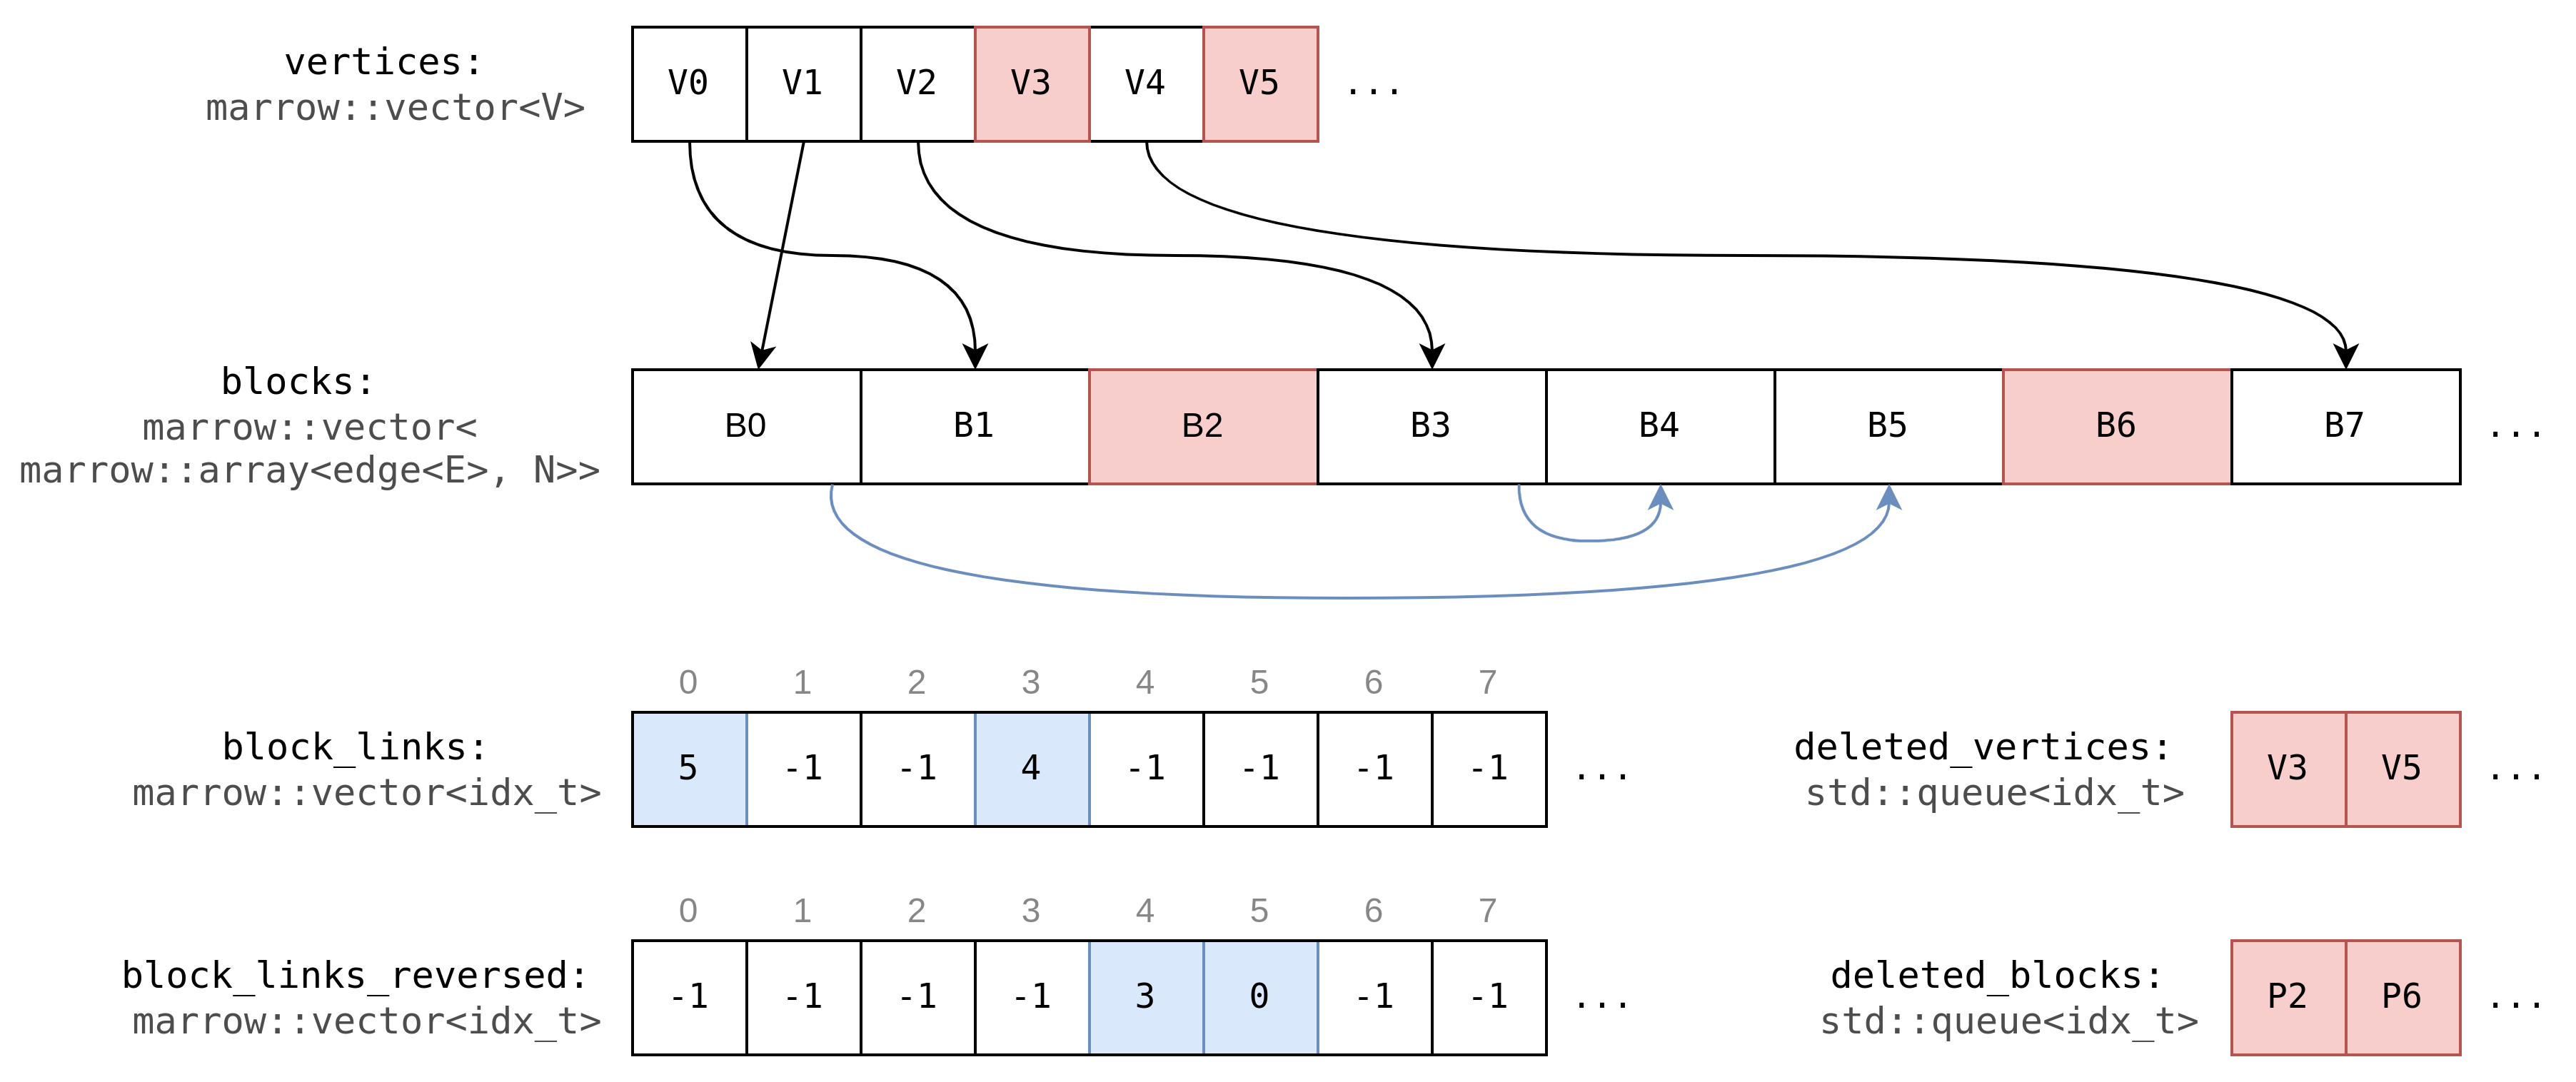
\includegraphics[width=\textwidth]{Chapters/Figures/Images/marrow_graph_data_struct.png}
    \caption{Marrow-Graph's data-structure.}
\label{fig:mg2_data_struct}
\end{figure}


\section{Algorithms}

Additionally to the previous basic operators, we plan to include a large suite of algorithms in Marrow-Graph. Gunrock already disposes of a large number of algorithms, written using the previously described programming model, which will be used as a basis for our own implementations. We will start by implementing \gls{SSSP}, \gls{BFS} and PageRank, given that these algorithms are commonly used for performance assessment, and follow from there.
